\documentclass[conference]{IEEEtran}
\IEEEoverridecommandlockouts
% The preceding line is only needed to identify funding in the first footnote. If that is unneeded, please comment it out.
\usepackage{cite}
\usepackage{amsmath,amssymb,amsfonts}
\usepackage{algorithmic}
\usepackage{graphicx}
\usepackage{textcomp}
\usepackage{xcolor}
\def\BibTeX{{\rm B\kern-.05em{\sc i\kern-.025em b}\kern-.08em
    T\kern-.1667em\lower.7ex\hbox{E}\kern-.125emX}}
\begin{document}

\title{Network packet generation for Artificial Intelligence\\
}

\author{\IEEEauthorblockN{ Bernhard Gally}
\IEEEauthorblockA{\textit{IT Security} \\
\textit{FH Technikum Wien}\\
Vienna, Austria\\
cs19m023@technikum-wien.at}
\and
\IEEEauthorblockN{Maximilian Wech}
\IEEEauthorblockA{\textit{IT Security} \\
\textit{FH Technikum Wien}\\
Vienna, Austria\\
cs19m020@technikum-wien.at}
}

\maketitle

\begin{abstract}
Supervised learning in artificial intelligence requires a training dataset that is already labeled. Doing so with network packets is a challenge due to the fact that even Intrusion Detection Systems are not always correct with their guessing. To overcome this problem it is necessary to generate malicious and benign packets and label them accordingly. To increase the quality of the dataset the IP addresses from the machines should not remain the same for all of the data and the malicious and benign traffic should be mixed. Therefore, a literature search is carried out in the relevant specialist literature, scientific work and publications in order to research the necessary basics. Different types of attacks, tools for carrying out attacks and how realistic network traffic can be generated are to be determined. The results show that some approaches exist to divide the multitude of different attack methods into a few, individual groups. Nine generic attack classes as well as typical attack targets and vulnerabilities are identified. In addition, various tools for carrying out attacks are determined. These can be divided into the areas of information gathering and attack launching. Furthermore, different strategies are considered to generate realistic network traffic consisting of benign and malicious data packets. In conclusion, the information determined in the context of this work helps to generate an appropriate dataset for supervised machine learning.
\end{abstract}

\begin{IEEEkeywords}
artificial intelligence, neural networks, computer networks, network security, packet generation
\end{IEEEkeywords}

\section{Introduction}
Generating network traffic that can be used to train a neural network brings some challenges: there are many different attack types that need to be considered, a vast variety of attack tools to generate malicious traffic, each with their own advantages and disadvantages, and realistic benign network traffic has to be generated, just to name a few.

This paper is split into three chapters. The first chapter explains the different kinds of attacks and their targets. The second chapter focuses on tools to generate malicious traffic. The third chapter addresses the problem of generating realistic network traffic. 

At this point all of our considerations are based on theoretical research without practical implementation which will come to life in further work. Therefore this paper sets a direction and foundation for the next steps and shows possible solutions at a high level. The results are elaborated on the basis of an extensive literature search in relevant specialist literature, scientific works and publications. The list of individual sources can be found at the end of the work.

\section{Cyber-attacks: types, targets, vulnerabilites}
\label{sec:cattv}

This chapter intends to provide an overview of various types of cyber-attacks, cyber-attack targets and exploitable vulnerabilities. 

\subsection{General information}
In order to fulfil the task, it initially appears necessary to describe typical characteristics of attacks. Attacks aim to exploit weaknesses, such as poorly configured systems, or errors in software and to circumvent security measures. Attackers deliberately try to make services unavailable, spy on or manipulate data and disrupt normal traffic as much as possible \cite{b1}. Executing attacks generally consists of several steps: First, the attacker's motivation must be clarified (e.g. proof of the attacker's own abilities). Then it is necessary to select a target and collect information about it. As soon as this has happened, the attack method is selected and the attack is performed \cite{b2}. 

\subsection{Classifying attacks}

\medskip Basically, there are too many different cyber-attack methods to mention all of them. Therefore, various approaches exist in the literature to classify attacks into different groups. One way is to split attacks into active and passive ones \cite{b3,b4}.  In the case of passive attacks, attempts are not made to manipulate data in network traffic, but rather to eavesdrop and collect sensitive information. The opposite is the case with active attacks, which attempt to manipulate network packets, for example \cite{b4}. 

At this point it also appears necessary to address the distinction between computer and network attacks mentioned in \cite{b2}. Computer attacks are spoken of when a computer system is attacked in any way. For example, attempts are made to slow down the performance of PCs or to manipulate data on hard disks. Network attacks are divided into two variants: The first option is to use the network to attack a computer system. Although these are network attacks, they can also be seen as a subset of computer attacks. The second option is when network attacks are actually directed only at the network and not at computer systems, for example by congesting a network with packets. The following figure is included to provide clarity and shows the relationship between computers and network attacks.

\begin{figure}[htbp]  
\centerline{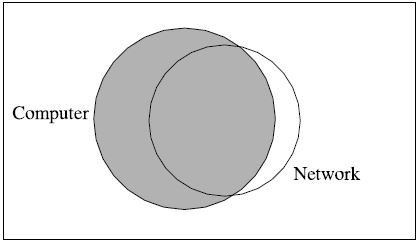
\includegraphics{computer-network-attacks.jpg}}
\caption{Relationship of computer and network attacks \cite{b2}}
\end{figure}

\medskip Further approaches exist such as classifying into internal and external attacks, or classifying attacks based on the underlying OSI-layer.

\medskip The classification model presented in \cite{b5}, which works on the basis of four dimensions and offers a holistic view of attacks, is often cited in the literature. First, an attack class is assigned based on the attack vector. The attack's target is specified in the second dimension. The vulnerabilities that are exploited by the attack are then noted. Finally, the fourth dimension analyses whether an attack has a payload or an effect that exceeds the typical characteristics of the type of attack \cite{b5} . The rest of this chapter will focus on further introducing this model and consider each dimension individually.

\subsubsection{First dimension}

\medskip As already mentioned, in the first dimension the attack class is determined on the basis of the attack vector. The following generic classifications are listed in \cite{b5}:

\smallskip Virus: this is a malware that replicates itself and, for example, infects other script code. When the infected source code is executed, the virus is also executed \cite{b6}.  Basically there are many different types of viruses. An example would be File Infectors, in which a virus is embedded in a file. If this file is executed, the virus is also executed \cite{b2}.

\smallskip Worms: a software that spreads independently by exploiting vulnerabilities \cite{b6}. Examples include mass mailing worms, which spread via email, and network-aware worms, which require only a few steps to infect a foreign host and spread themselves \cite{b2}.

\smallskip Trojans: a software that appears harmless at first, but also contains a hidden, malicious function \cite{b6}. One example are logic bombs, which only execute their malicious payload when a specific condition (e.g. a certain time of a day) has been reached \cite{b2}.

\smallskip Buffer overflows: This type of attack is based on programming errors and is very often used to attack computers or networks. Principally an attempt is made to overfill a temporary memory area. The amount of data that exceeds the size of the memory overwrites and corrupts other data. One possible goal of this attack would be to take control of a process. The main types of this attack are stack and heap buffer overflows \cite{b2}.

\smallskip Denial of service attacks: this means attacks on the availability of systems.  An attempt is made to exhaust the resources required to run a service \cite{b6}. This attack can be host-based, network-based, or distributed. The latter version is a DDoS attack, in which several attackers attack a mutual target at the same time \cite{b2}.

\smallskip Network attacks: the category is divided into several sub-areas. If an attacker pretends to be someone else by manipulating certain addresses, this is called spoofing. This can take place on the basis of the MAC address (MAC Address Spoofing) or on the basis of the IP address (IP Spoofing). An attack in which IP spoofing is used is session hijacking. Here, an attacker tries to link into a session (based, for example, on TCP / Telnet) between two hosts and virtually replace one host. In the case of wireless network attacks, weaknesses such as too short initialization vectors of the WEP standard can be exploited. In the event of attacks on web applications, attempts are made to exploit security gaps in them.  For example, if there is no strict separation between user input and program instructions, or there is insufficient input validation, an attacker can successfully send manipulated SQL statements to the underlying database. The consequences would be spying out of data or losing control of the underlying server. \cite{b2}.

\smallskip Physical attacks: this type of attack aims to cause physical damage to target systems (i.e. computers or networks). This includes, for example, deliberately cutting network cables or destroying computers \cite{b2}.

\smallskip Password attacks: here an attempt is made to find out a specific password in order to gain control over a PC, for example. This can be done in three different ways: trying out all possible password combinations (brute force), trying out a part of all possible password combinations (e.g. testing simple passwords) and determining deficiencies in password storage / encryption \cite{b2,b5}.

\smallskip Information gathering attacks: this type of attack does not change data; it is only about spying on (sensitive) information, which can be used for follow-up attacks \cite{b5}. A possible variant of this is sniffing of packets, to find out about IP and MAC addresses or passwords \cite{b2}.

\medskip \subsubsection{Second dimension}The targets of attacks are described in the second dimension of the classification model. These should be described as specifically as possible, which means that it is not sufficient, for example, to specify which server was attacked, but rather which service or which operating system is affected with which version. It should also be noted that an attack can target more than one target. Basically three groups of attack targets are defined \cite{b5}:

\smallskip Hardware: this group is divided into three areas. First of all, computers and their components (e.g. processors, random access memory) should be mentioned. Network devices such as routers or switches also belong to this category. Ultimately, peripheral devices such as monitors and keyboards are also included.

\smallskip Software: here a distinction is made between targets on operating systems (Windows, Linux, etc.) and various applications (email client, text processing program) that are executed on an operating system.

\smallskip Network: in this group, the target is not software or hardware but the network itself, or an associated network protocol (for example, TCP).

\medskip \subsubsection{Third dimension}In the third dimension of the classification model \cite{b5}, vulnerabilities that can be exploited by attacks are considered. Reference is made to the industry standard CVE - Common Vulnerabilities and Exposures \cite{b7}, which is used for the uniform naming of security gaps and vulnerabilities in computer systems. General vulnerability types are also defined in\cite{b8}:

\smallskip Implementation: if a system is not implemented according to the design, security gaps arise.

\smallskip Design: an incorrect design leads to a security-threatening implementation.

\smallskip Configuration: If a system is not configured correctly, doors are opened to the attackers.

\medskip \subsubsection{Fourth dimension}The last dimension analyzes whether an attack has a payload or an effect that exceeds the typical characteristics of the type of attack. This should result in a detailed view of the payload. For example, a worm's payload might be a Trojan, or the worm might just be manipulating files \cite{b5}.

\medskip The classification model offers a comprehensive view of attacks. For example, for a worm that is distributed via email (dimension 1), the target Windows 95 (dimension 2) with an inadequate configuration (dimension 3) and a virus as payload (dimension 4) could be determined. Further dimensions could be specified, for example what damage is caused by an attack, or how many costs arise from successfully carrying out the attack. Overall an overview is provided of how attacks can be classified, which attack targets are possible, or which vulnerabilities exist.


\section{Tools}

There is a large number of network tools available in the world wide web. Many of them are free to download and can be used for malicious activities but there are also many that can be used for defensive purposes. Generally speaking there are two major groups: tools for network attackers and tools for network defenders.\cite{b1} The tools for network attackers are the ones generating the packets thus being the ones we will focus on. 

\begin{figure}[htbp]  
\centerline{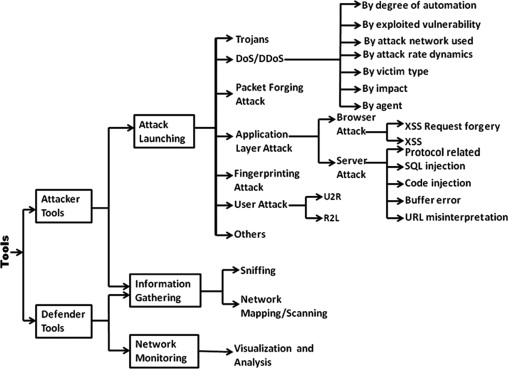
\includegraphics[scale=.65]{network-tools.jpg}}
\caption{Taxonomy of network security tools \cite{b1}}
\end{figure}

\subsection{Information gathering}
Attackers usually collect information before starting their attack. Understanding the environment, what operating systems are used, finding open ports and available services are only a small part of information that can be obtained. 

\smallskip Table \ref{table:sniffing-tools} contains a list of sniffing tools that are available online. Generally speaking, sniffing tools do not generate packets and are therfore undetectable. However, on a switched ethernet network segment a sniffer does generate a small amount of packets such as ARP\cite{b9}. Other types of sniffers, such as Ettercap, can execute a Man-in-the-middle attack. This causes a lot of packets to be sent through the network as it needs to answer requests in order to spoof an identity.

\begin{table}[htbp]
\caption{Sniffing tools \cite{b1}} 
\centering
\begin{tabular}{ | c | c | }
\hline
Tool name & Purpose \\
\hline
Ethereal & Packet capturing \\
Tcpdump & Packet capturing  \\
Net2pcap & Packet capturing  \\
Snoop & Packet capturing \\
Angst & Sniffing  \\
Ngrep & Capturing packet  \\
Ettercap & Man-in-the-middle attack  \\
Dsniff & Password sniffing  \\
Cain \& able & Password recovery  \\
Aimsniff & Capturing packet \\
Tcptrace & Analysis of traffic \\
Tcptrack & TCP connection analysis  \\
Argus & Analysis of audit data \\
Karpski & Packet analyzer \\
IPgrab & Display packet header \\
Nast & Traffic analysis \\
Gulp & Packet capturing/visualization \\
Libpcap & Packet capturing \\
Nfsen & Flow capturing/ visualization \\
Nfdump & Flow capturing/visualization \\
\hline
\end{tabular}
\label{table:sniffing-tools}
\end{table}

Scanning tools are often more intrusive than sniffing tools and generate lots of packets that can be detected. Their aim is to show up open ports, available services, used operating systems. With the gathered information an attacker can pick a suitable attack vector.
Table \ref{table:scanning-tools} shows a few common network scanning tools. 

\begin{table}[htbp]
\caption{Scanning tools \cite{b1}} 
\centering
\begin{tabular}{ | c | c | }
\hline
Tool name & Purpose \\
\hline
Nmap & Scanning	 \\
Amap & Scanning \\
Vmap & Version mapping \\
Unicornscan & Scanning \\
Ttlscan & Scanning \\
Ike-scan & Host discovery \\
Paketto & Scanning \\
\hline
\end{tabular}
\label{table:scanning-tools}
\end{table}

\subsection{Attack launching}
The most packets, however, are generated by the attacks themselves.
Especially some kinds of DoS attacks are designed to overload the network with packets so that the victim cannot respond to legitimate requests. 

\subsubsection{Denial of service}
The Internet provides many tools that are capable of executing DoS attacks and can be easily used to crash hosts or even networks.
Two examples of such tools are Low Orbit Ion Cannon (LOIC) or High Orbit Ion Cannon (HOIC). Both of these tools are capable of launching DoS/DDoS attacks within a short amount of time.
LOIC supports TCP, UDP and HTTP whereas HOIC only supports the HTTP protocol\cite{b1}. A list of DoS and DDoS tools is shown in Table \ref{table:ddos-tools}.

\begin{table}[htbp]
\caption{DoS/DDoS tools \cite{b1}} 
\centering
\begin{tabular}{ | c | c | }
\hline
Tool name & Purpose \\
\hline
Jolt & DoS \\
Burbonic & DoS \\
Targa & DoS \\
Blas20 & DoS \\
Crazy Pinger & DoS \\
UDPFlood & DoS \\
FSMax & DoS \\
Nemsey & DoS \\
Panther & DoS \\
Land \& LaTierra & DoS \\
Slowloris & DoS \\
Blackenergy & DDoS \\
HOIC & DDoS \\
Shaft & DDoS \\
Knight & DDoS \\
Kaiten & DDoS \\
RefRef & DDoS \\
Hgod & DDoS \\
LOIC & DDoS \\
Trinoo & DDoS \\
TFN & DDoS \\
TFN2K & DDoS \\
Stachaldraht & DDoS \\
Mstream & DDoS \\
Trinity & DDoS \\
\hline
\end{tabular}
\label{table:ddos-tools}
\end{table}

\smallskip
\subsubsection{Packet forging}
Packet forging tools are necessary to manipulate packet information. With the help of such tools it is possible to generate traffic with non-existant IP addresses. They also allow to individually set the flags of network packets to a desired state. An extreme example of such a packet is the "Christmas tree packet", which has all available flags set to 1. A list of packet forging tools is shown in Table \ref{table:packetforging-tools}.


\begin{table}[htbp]
\caption{Packet forging tools \cite{b1}} 
\centering
\begin{tabular}{ | c | c | c |}
\hline
Tool name & Purpose \\
\hline
Packeth & Packet generator	 \\
Packit & Packet analysis and injection	 \\
Nemesis & Packet crafting/injection	 \\
Tcpinject & Packet generator	 \\
Libnet & Packet injection	 \\
SendIP & Packet generator	 \\
IPsocery & Packet generator	 \\
Pacgen & Packet generator	 \\
Arp-sk & ARP packet generator	 \\
ARP-SPOOF & Packet intercept	 \\
Libpal & Packet intercept	 \\
Aicmspend & ICMP packet flooding	\\
\hline
\end{tabular}
\label{table:packetforging-tools}
\end{table}

\smallskip
\subsubsection{Application layer}
Application layer attacks use legitimate requests to use up all the resources of the victim. Unlike DDoS attacks, they are more subtle and more difficult to detect since they are using legitimate requests. 

\smallskip
\section{Generating a realistic network load}
A problem that exists with generating a realistic network load is the unwanted burstiness of real networks. Misconfigurations can result in traffic that looks similar to flooding attacks \cite{b10} and are hard to reproduce in small sandbox networks. Existing datasets often do not include such noise which result in unrealistic datasets \cite{b10}.
 
\smallskip According to \cite{b10} it might be impossible to create a single representative background trace that contains benign and malicious traffic. The reason is that the expected traffic workload and characteristics are highly dependent on the network and its hosts.

Tools such as Trident provide multiple strategies to create benign traffic \cite{b10}. 

\subsection{NIDS-based strategies}
Using a wellknown network intrusion detection system (NIDS) such as Snort, these tools can groom a packet trace from a local site. This approach causes problems since benign packets that are flagged as malicious (false postives) are removed.

\subsection{Synthetic generation strategies}
Software robots emulate user behaviour and thus generate synthetic traffic. The idea behind it is that the robot only creates connections with known good hosts. 

\subsection{Trust-based strategies}
The third strategy they support is by grooming a packet trace taken at a local site using connection heuristics. Examples of these heuristics are failure rates or scanning characteristics. This approach makes use of different connection characteristics of malicious and benign sources based on a model of malicious connection behaviour \cite{b10}.
The advantage of using this strategy is that it is not influenced by a particular system (NIDS independence) and is based on transport level characteristics. The disadvantage is that a connection that is sufficiently similar to benign users will not be detected.



\section{Summary and conclusion}
Various aspects must be taken into account for the generation of realistic network traffic for the production of a dataset, which is subsequently used for supervised machine learning. In the course of this paper, cyber-attacks were explained in principle, various tools for carrying out the attacks were shown, and how realistic network traffic based on benign and malicious data packets can be generated. The topics covered are summarized at this point in order to emphasize the most important content again.

Cyber -attacks generally try to exploit various vulnerabilities and carry out malicious actions. In order to provide an overview of the multitude of different attack methods, there are various approaches in the literature to classify the attacks into a few groups. The focus of this work is the classification model found in  \cite{b5}, which aims to enable a holistic view of attacks. Basically, nine different attack classes are described, including network attacks, denial of service attacks, information gathering attacks and various types of malware-based attacks. Subsequently, various attack targets (software, hardware and network), as well as vulnerabilities (in design, implementation, configuration) are explained in more detail.
Tools for carrying out-cyber attacks are basically divided into two different groups, namely information gathering tools and attack launching tools. The former tries to find out various information about the system to be attacked (open ports, operating system used, etc.). Sniffing and scanning tools can be used for this. Attack launching tools for performing denial of service attacks and for packet forging were identified. Furthermore, it is also possible to proceed on the basis of legitimate requests on the application layer. The creation of realistic network traffic based on benign and malicious data packets is a complex undertaking. By using tools, various strategies exist to generate harmless traffic, for example by using software robots.

\section{Further research}
Future work on this topic could try to look at attack methods on a more detailed level in order to provide more specific information. Furthermore, it makes sense to identify additional tools for carrying out cyber-attacks. There is also room for further research in the search for other ways of generating realistic network traffic including benign and malicious behavior. 

\begin{thebibliography}{00}
\bibitem{b1} N. Hoque, M. H. Bhuyan, R. C. Baishya, D. K. Bhattacharyya und J. K. Kalita, ``Network attacks: Taxonomy, tools and systems'', Journal of Network and Computer Applications, 2014. Jg., Nr. 40, 2014.
\bibitem{b2} S. Hansman,  ``A Taxonomy of Network and Computer Attack Methodologies'', 2003.
\bibitem{b3} M. W. Pawar and J. Anuradha,  ``Network Security and Types of Attacks in Network'', Procedia Computer Science,  Nr. 48, 2015.
\bibitem{b4} A. Gagandeep and K. Pawan,  ``Analysis of Different Security Attacks in MANETs on Protocol Stack A-Review'', International Journal of Engineering and Advanced Technology (IJEAT), 2012.
\bibitem{b5} S. Hansman and R. Hunt,  ``A taxonomy of network and computer attacks'', Computers \& Security, Nr. 24, 2004.
\bibitem{b6} W. Stallings und L. Brown,  ``Computer Security: Principles and Practice'',  3rd Ed., 2015.
\bibitem{b7} Common Vulnerabilities and Exposures. [Online] Available at: https://cve.mitre.org/.
\bibitem{b8} J. D. Howard,  ``An Analysis Of Security Incidents On The Internet'', 1995.
\bibitem{b9} R. Spangler, ``Packet Sniffer Detection with AntiSniff'', 2003
\bibitem{b10}  J. Sommers, V. Yegneswaran and P. Barford. ``Toward Comprehensive Traffic Generation for Online IDS Evaluation''. Technical report, Dept. of Computer Science, University of Wisconsin, August 2005.
\end{thebibliography}




\end{document}
